%------------------------------------------------------------------------------
% Document class
%------------------------------------------------------------------------------

\documentclass[conference]{IEEEtran}
\usepackage[lastpage,user]{zref}


%------------------------------------------------------------------------------
% Packages
%------------------------------------------------------------------------------
\usepackage[utf8]{vietnam}
\usepackage{graphicx}
\usepackage[breaklinks=true]{hyperref}
\usepackage{amsmath}
\usepackage{listings}
\usepackage{color}

\definecolor{dkgreen}{rgb}{0,0.6,0}
\definecolor{gray}{rgb}{0.5,0.5,0.5}
\definecolor{mauve}{rgb}{0.58,0,0.82}

\lstset{frame=tb,
  language=Java,
  aboveskip=3mm,
  belowskip=3mm,
  showstringspaces=false,
  columns=flexible,
  basicstyle={\small\ttfamily},
  numbers=none,
  numberstyle=\tiny\color{gray},
  keywordstyle=\color{blue},
  commentstyle=\color{dkgreen},
  stringstyle=\color{mauve},
  breaklines=true,
  breakatwhitespace=true,
  tabsize=3
}

\usepackage{booktabs,dcolumn}
\newcolumntype{d}[1]{D{.}{.}{#1}} % "decimal" column type
\renewcommand{\ast}{{}^{\textstyle *}} % for raised "asterisks"

%------------------------------------------------------------------------------
% Hyphenation
%------------------------------------------------------------------------------
\hyphenation{op-tical net-works semi-conduc-tor}
\newcommand\tab[1][1cm]{\hspace*{#1}}

%------------------------------------------------------------------------------
% Begin of document
%------------------------------------------------------------------------------
\begin{document}


%------------------------------------------------------------------------------
% Header of document
%------------------------------------------------------------------------------
% Title
\include{Abbr}
\title{Nhận dạng khuôn mặt dùng thuật toán SIFT }

\author{
\IEEEauthorblockN{
Nguyễn Văn Quảng\IEEEauthorrefmark{1},
Bùi Thanh Tính\IEEEauthorrefmark{1},
Nông Thành Nam\IEEEauthorrefmark{1},
Nguyễn Việt Phú\IEEEauthorrefmark{1},
Bùi Vũ Viết Phương\IEEEauthorrefmark{1} 
} 
\IEEEauthorblockA{\IEEEauthorrefmark{1} Môn học Xử Lý Ảnh \\ Khoa Điện - Điện tử \\ Đại học Bách Khoa TPHCM\\
		Email: \{1512670, 1513505, 1512099, 1512493, 1512568\}@hcmut.edu.vn}
}
\maketitle


%------------------------------------------------------------------------------
% Commands
%------------------------------------------------------------------------------
\providecommand{\keywords}[1]{\textbf{\textit{    Từ khóa---}} #1}


%------------------------------------------------------------------------------
% Abstract
%------------------------------------------------------------------------------
\begin{abstract}
Trong bài báo cáo này, nhóm em đã nghiên cứu về thuật toán SIFT và ứng dụng của nó: nhận dạng khuôn mặt. Scale-Invariant Feature Transform (SIFT) là phương pháp dùng để trích xuất các điểm đặc trưng từ bức ảnh \cite{baibao1}, là giải thuật trong lĩnh vực Computer Vision. Giải thuật này đã được giới thiệu bởi David Lowe năm 1999. SIFT đã được ứng dụng trong nhiều lĩnh vực như nhận dạng khuôn mặt và nhận dạng đối tượng. Nhóm em đã tìm hiểu thuật toán SIFT bao gồm 4 bước chính để nhận dạng và miêu tả điểm đặc trưng (local features) trong ảnh. Thêm nữa, nhóm em đã dùng dùng phương pháp tính khoảng cách Euclide (Euclidean distance) như là một giải thuật để so sánh các điểm đặc trưng mục đích để nhận dạng với nhau.
\end{abstract}

\keywords{SIFT, nhận dạng khuôn mặt (Face Recognition), nhận dạng đối tượng (Object Recognition), so khớp ảnh (Image Matching) và khoảng cách Euclide (Euclidean distance).}

\IEEEpeerreviewmaketitle


%------------------------------------------------------------------------------
% Section 1: Introduction
%------------------------------------------------------------------------------
\medskip
\section{Giới thiệu}
\subsection{Tác giả}
David G. Lowe (hình \ref{fig:tacgia}) là một nhà khoa học máy tính của Canada, làm việc cho Google với tư cách là một nhà nghiên cứu chuyên sâu (senior) trong the Machine Intelligence Group. Ông là cựu giáo sư khoa Khoa học máy tính tại đại họa British Columbia và đại học New York.


Ông là một nhà nghiên cứu trong lĩnh vực Computer Vision, nhận dạng đối tượng và các mô hình tính toán về human vision. Ông là tác giả của thuật toán SIFT, một trong những thuật toán phổ biến nhất dùng để phát hiện và mô tả đặc trưng của bức ảnh.
\begin{figure}
  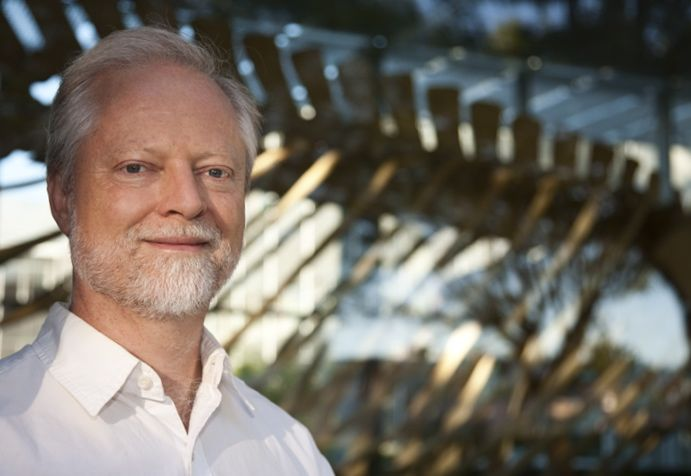
\includegraphics[width=\linewidth]{tacgia}
  \caption{David G. Lowe}
  \label{fig:tacgia}
\end{figure}
\subsection{Giới thiệu thuật toán SIFT}

Scale-Invariant Feature Transform (SIFT) là giải thuật trong lĩnh vực Computer Vision, dùng để nhận dạng và miêu tả những điểm đặc trưng (local features) trong ảnh. Giải thuật lần đầu được giới thiệu bởi David Lowe năm 1999. Giải thuật này (cùng với giải thuật anh em là SURF) được ứng dụng rộng rãi trong Nhận dạng đối tượng (object recognition), mô hình hóa 3D (3D modeling),...

    Điểm đặc biệt của SIFT nằm ngay trong cái tên của nó Scale-Invariant, tức là nó sẽ đưa ra các kết quả ổn định với những scale của ảnh khác nhau, bên cạnh đó cũng có thể nói giải thuật này có tính rotation-invariant.
    
Phần còn lại của bài báo cáo được tổ chức như sau. Trong phần~\ref{Sec:GiaiThuatSIFT} và phần~\ref{Sec:PhuongPhapMatching}, nhóm em lần lượt trình bày mô hình và phân tích thuật toán SIFT cũng như phương pháp khớp nối ảnh. Trong phần~\ref{Sec:Cacdactinh}, nhóm em sẽ kiểm chứng các kết quả phân tích bằng các kết quả mô phỏng trên phần mềm Matlab. Cuối cùng, nhóm em kết luận bài báo trong phần~\ref{Sec:KetLuan}.


%------------------------------------------------------------------------------
% Section 2: System overview
%------------------------------------------------------------------------------
\medskip
\section{Giải thuật SIFT}
\label{Sec:GiaiThuatSIFT}
%\cite{AndroidServClient}
Ở phần này, nhóm em trình bày tổng quan về bộ mô tả SIFT. Giải thuật SIFT biến đối dữ liệu hình ảnh thành điểm đặc trưng mà bất biến với tỉ lệ. Trong bài báo khoa học "Distinctive Image Features from Scale-Invariant Keypoints" \cite{baibao1}, SIFT được đặc tả rõ nét dưới bốn giai đoạn (stages) chính sau:\\
    • Scale-space extrema detection.\\
    • Keypoint localization.\\
    • Orientation assignment.\\
    • Keypoint descriptor.\\
Sau đây, nhóm em sẽ trình bày tư tưởng chung của từng giai đoạn:
\subsection{Scale-space extrema detection}
Giai đoạn đầu tiên của tìm kiếm được tính trên tất cả các tỉ lệ và vị trí hình ảnh. Nó được thực hiện hiệu quả bằng cách sử dụng hàm DoG(Difference-of-Gaussian) để xác định các điểm quan tâm tiềm năng, đó là những điểm bất biến với các tỉ lệ và hướng.


Để thực hiên giai đoạn đầu tiên: cách tìm Scale-space đã được chứng minh bởi Koenderink (1984) và Lindeberg (1994) mà theo một loạt các  giả định hợp lý, hạt nhân không gian quy mô duy nhất có thể là hàm Gaussian (bộ lọc gaussian làm mờ ảnh).

Do đó, Scale-space của một hình ảnh được định nghĩa là một hàm, ${L(x,y,\sigma)}$, được tạo ra từ sự biến đổi của Gaussian, ${G(x,y,\sigma)}$, với một hình ảnh đầu vào, ${I(x,y)}$:
\begin{equation}
L(x,y,\sigma) = G(x,y,\sigma) * I (x, y)
\end{equation}

Trong đó $*$ là phép toán nhân chập giữa $x$, $y$ và $\sigma$:
\begin{equation}
G(x,y,\sigma) = \frac{1}{2 \pi \sigma^2}\mathrm{e}^{-(x^2+y^2)/2\mathrm{e}^2}\
\end{equation}


Để phát hiện địa điểm Keypoint ổn định và hiệu quả trong không gian tỉ lệ, Lowe đã đề xuất sử dụng không gian cực trị dùng hàm difference-of-Gaussian với các hình ảnh ${D(x, y, \sigma)}$, chúng có thể được tính toán từ sự khác biệt của hai tỉ lệ lân cận cách nhau bởi một số hằng số k không đổi.
\begin{equation}
D(x,y,\sigma) = G(x,y,k\sigma) - G(x,y,\sigma)*I(x,y) 
\end{equation} 
\begin{equation}
\Rightarrow D(x,y,\sigma) = L(x,y,k\sigma) - L(x,y,\sigma)
 \end{equation}
Có một số lý do cho việc lựa chọn hàm này. Đầu tiên nó là một hàm đặc biệt về hiệu suất để tính toán như những hình ảnh mịn L cần phải được tính toán trong bất kỳ bộ mô tả thuộc tính không gian tỉ lệ nào và D có thể được tính bằng cách đơn giản là trừ hình ảnh (hình \ref{fig:hinh2_phu}).
\begin{figure}
  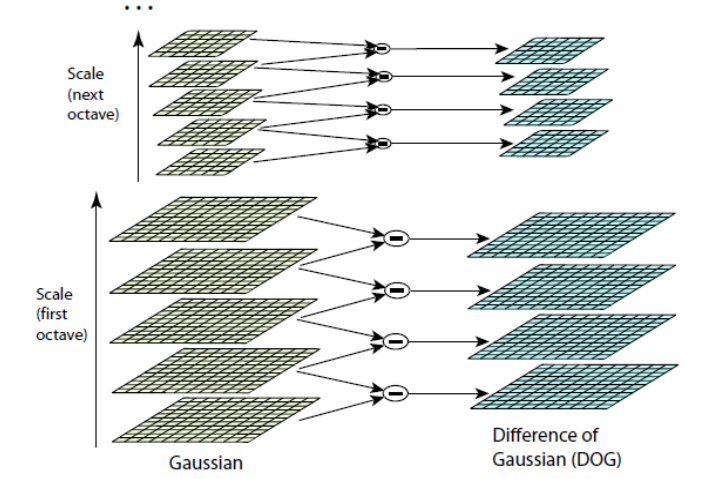
\includegraphics[width=\linewidth]{hinh2_phu}
  \caption{Mô tả hàm Gaussian và hàm Difference-of-Gaussian (DoG)}
  \label{fig:hinh2_phu}
\end{figure}

Ngoài ra, các hàm Gaussian khác nhau cung cấp một xấp xỉ gần Laplacian tỉ lệ. Bình thường Laplacian of Gaussian là ${\sigma^2\nabla^2G}$ như nghiên cứu bởi Lindeberg (1994). Lindeberg cho thấy rằng Laplacian bình thường với các yếu tố ${\sigma^2}$ là thực sự cần thiết cho tỉ lệ bất biến. Các cực đại và cực tiểu của ${\sigma^2\nabla^2G}$ tạo nên các thuộc tính hình ảnh ổn định nhất so với một các hàm hình ảnh khác chẳng hạn như gradient, Hessian hoặc hàm của góc Harris(trong so sánh thử nghiệm chi tiết Mikolajczyk (2002)). Mối quan hệ giữa D và ${\sigma^2\nabla^2G}$ như sau:
\begin{equation}
\frac{dG}{d\sigma} = \sigma\nabla^2G
\end{equation}

Từ đây, chúng ta thấy rằng $\nabla^2G$ có thể được tính xấp xỉ để $\frac{dG}{d\sigma}$ đạt sự khác biệt gần nhất về tỉ lệ tại $k\sigma$ và $\sigma$:
\begin{equation}
\sigma\nabla^2G = \frac{dG}{d\sigma} \approx \frac{G(x,y,\sigma) - G(x,y,\sigma)}{k\sigma - \sigma}
\end{equation}

và do đó,
\begin{equation}
G(x,y,\sigma) - G(x,y,\sigma) \approx (k-1)\sigma^2\nabla^2G
\end{equation} 

Điều này cho thấy rằng khi các hàm khác của hàm Gaussian có tỉ lệ khác nhau bởi một hằng số có quan hệ chặt chẽ với tỉ lệ ${\sigma^2}$ cho tỉ lệ bất biến Laplacian. Các yếu tố ${(k-1)}$ trong phương trình là một hằng số trên tất cả tỉ lệ và do đó không ảnh hưởng đến vị trí cực trị. Các lỗi xấp xỉ sẽ trả về 0 khi k tiến đến 1, nhưng trong thực tế, người ta đã tìm thấy rằng xấp xỉ gần như không có tác động đến sự ổn định của việc phát hiện cực trị hoặc địa phương hóa đối với sự khác biệt quan trọng về tỉ lệ, như ${k=\sqrt{2}}$. (hình \ref{fig:hesok_phu})
\begin{figure}
  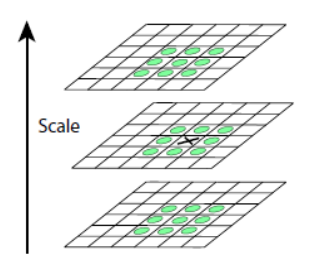
\includegraphics[width=\linewidth]{hesok_phu}
  \caption{Phát hiện cực trị của hàm DoG}
  \label{fig:hesok_phu}
\end{figure}

Phát hiện cực trị địa phương: Để phát hiện cực đại và cực tiểu địa phương của $D{(x, y, \sigma)}$, mỗi điểm mẫu được so sánh với tám điểm láng giềng của bức ảnh hiện tại và chín điểm láng giềng ở tỉ lệ trên và dưới. Nó được chọn khi và chỉ khi nó lớn hơn tất cả các nước láng giềng hoặc nhỏ hơn tất cả. Chi phí của việc kiểm tra này là khá thấp do thực tế hầu hết các điểm lấy mẫu sẽ được loại bỏ sau lần đầu kiểm tra.

$\bullet$ Để xác định tần số lấy mẫu cho mỗi $octave$ của không gian tỉ lệ thì phải xác định tần số lấy mẫu trong hình ảnh liên quan đến tỉ lệ của độ mịn. Giả sử rằng cực trị có thể được tự ý gần nhau, sẽ có một sự hoán đổi tương tự giữa tần số lấy mẫu và tỷ lệ phát hiện. Hình \ref{fig:thutulammin_phu} cho thấy thực nghiệm của lượng làm mịn trước khi $\sigma$ được áp dụng cho từng cấp hình ảnh trước khi xây dựng các không gian biểu diễn tỉ lệ cho một $octave$. Dòng trên cùng là lặp lại của phát hiện keypoint và kết quả cho thấy rằng khả năng lặp lại tiếp tục tăng với $\sigma$. Tuy nhiên, nếu chọn $\sigma$ quá lớn thì lại mất nhiều thời gian, để tăng hiệu quả ta lựa chọn $\sigma = 1.6$ cung cấp gần lặp lại tối ưu. 

\begin{figure}
  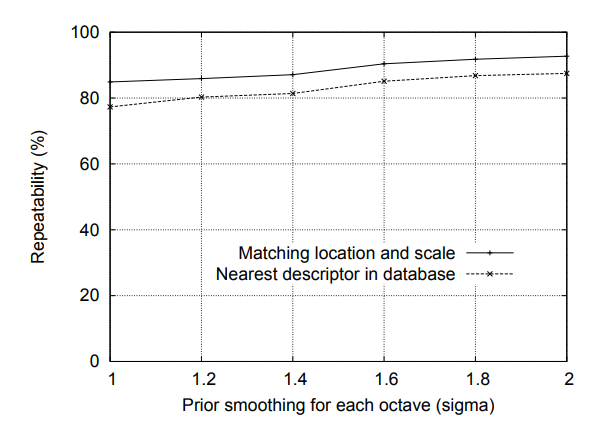
\includegraphics[width=\linewidth]{thutulammin_phu}
  \caption{Thứ tự làm mịn cho mỗi Octave}
  \label{fig:thutulammin_phu}
\end{figure}

Ví dụ: Hình ảnh ban đầu có một vệt mờ tối thiểu $\sigma = 0,5$ (mức tối thiểu cần thiết để ngăn chặn hiện tượng răng cưa tại đường biên ảnh), và do đó để tăng các điểm ảnh ta cần tăng gấp đôi giá trị $\sigma = 1,0$ Điều này có nghĩa rằng việc làm mịn bổ sung là cần thiết trước khi tạo ra các octave đầu tiên của không gian tỉ lệ. Việc tăng gấp đôi hình ảnh làm tăng số lượng các keypoint ổn định gần gấp 4.
\begin{figure}
  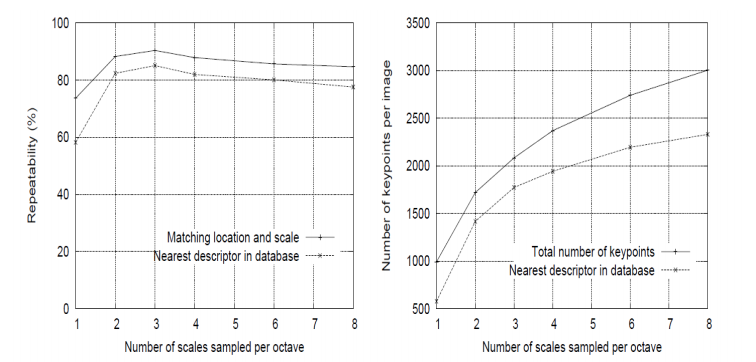
\includegraphics[width=\linewidth]{soluonglaymau_phu}
  \caption{Số lượng mẫu tỷ lệ trên mỗi Octave}
  \label{fig:soluonglaymau_phu}
\end{figure}
 
Như hình \ref{fig:soluonglaymau_phu} cho thấy, độ lặp lại cao nhất thu đựợc khi lấy mẫu 3 thang mỗi $octave$.

Số keypoint tăng lên với việc tăng tỉ lệ mẫu và tổng số các đối sánh đúng cũng tăng. Tuy nhiên, chi phí của việc tính toán cũng tăng lên với con số này, vì vậy mà ta lựa chọn sử dụng chỉ 3 mẫu tỉ lệ mỗi $octave$.

\subsection{Keypoint localization}
Vì ở bước 1 đã tạo ra quá nhiều keypoint candidates, trong số đó có thể có những keypoint không ổn định. Vì vậy ở bước thứ 2 này, ta sẽ thực hiện một bước chi tiết hơn đối với 3 yếu tố: vị trí (position), tỉ lệ (scale) và tỉ số đường cong chính (radio of principle curvatures). Thông tin này cho phép chúng ta loại bỏ những keypoint mà có độ tương phản thấp (ví dụ như nhiễu) và các điểm xấu được xác định ở phần rìa (poorly localized along an edge).\\


Các bước tiến hành:

	- Nội suy dữ liệu lân cận để tìm vị trí chính xác (Interpolation of nearby data for accurate position)
	
	
	- Loại bỏ các điểm có độ tương phản thấp (Discarding low-contrast keypoints)
	
	
	- Loại bỏ các điểm dư thừa theo biên (Eliminating edge responses)\\
	
	Ta sẽ đi sâu vào từng bước:
	
	\subsubsection{Nội suy dữ liệu lân cận}
Dựa trên phương pháp của (Brown and Lowe, 2002 \cite{baibao2}): xác định vị trí nội suy (interpolated location) của điểm cực trị. Mục đích của việc làm này là nâng cao được khả năng matching và tính ổn định (stability).
Việc nội suy được thực hiện bằng cách sử dụng chuỗi Taylor mở rộng cho hàm không gian tỉ lệ (Difference-of-Gaussian scale-space function $D(x, y, \sigma)$), trong đó candidate keypoint là điểm gốc. 
\begin{equation}
D(x) = D + \frac{\partial D^T}{\partial x}x + \frac{1}{2}x^T \frac{\partial^2 D}{\partial x^2}x
\end{equation}
Trong đó: D và các đạo hàm được đánh giá tại điểm lấy mẫu và ma trận $x= (x, y, \sigma )^T$

Vị trí của điểm cực trị $\hat{x}$: được xác định bằng cách lấy đạo hàm theo $x$ của hàm $D(x)$, ta được: 
\begin{equation}
\hat{x} = - \frac{\partial^2 D^{-1}}{\partial x^2}\frac{\partial D}{\partial x}
\end{equation}
Nếu ${\hat{x} \geq 0,5}$ với mọi kích thước thì ta suy ra được điểm cực trị nằm gần hơn các điểm lấy mẫu (keypoint candidate) khác. Trong trường hợp này, candidate keypoint ban đầu sẽ được thay đổi và việc nội suy sẽ được thực hiện. Giá trị của phần bù cuối cùng $\hat{x}$ sẽ được thêm vào candidate keypoint của nó để có được ước tính nội suy cho vị trí của cực trị.

	\subsubsection{Loại bỏ các điểm có độ tương phản thấp}
	
Sau khi có được điểm cực trị, giá trị của hàm $D(\hat{x})$ được dùng để loại bỏ $extrema$ không ổn định với độ tương phản thấp. Giá trị này được tính như sau: 
\begin{equation}
D(\hat{x}) = D + \frac{1}{2} \frac{\partial D^T}{\partial x} \hat{x}
\end{equation}
	
Theo bài báo của Lowe, D. 2004 \cite{baibao1}, tại tất cả các điểm cực trị có giá trị $D(\hat{x}) \leq  0.03$ sẽ bị loại bỏ. Vì các điểm này có độ tương phản thấp cũng như không ổn định. 
	\subsubsection{Loại bỏ các điểm dư thừa theo biên}
	
	Để ổn định hơn, ngoài việc loại trừ keypoint có độ tương phản thấp, ta còn phải loại trừ thêm các điểm dư thừa theo biên. Lý do của việc làm này là bởi vì hàm $DoG$ (Difference-of-Gaussian) có một đáp ứng biên rất mạnh dọc theo các rìa, vì vậy mà các điểm tại các rìa sẽ rất khó xác định và vì vậy sẽ không được ổn định khi có một lượng nhiễu nhỏ.

Vì vậy, để nâng cao khả năng ổn định, ta cần loại bỏ các điểm keypoint ở tại vị trí khó xác định nhưng lại có đáp ứng biên cao.

Trong hàm DoG, điểm đỉnh (peak) rất khó định nghĩa. Nhưng điểm đỉnh có một đường cong chính (principal curvatures) nằm dọc theo các rìa kèm theo là đường cong nhỏ nằm theo hướng vuông góc. Những đường cong chính này được xác định từ ma trận vuông $2x2$ Hessian, được tính tại vị trí và tỉ lệ của keypoint.

\begin{equation}
	H = \begin{bmatrix}
	D_{xx} 	& D_{xy} \\
	D_{xy} 	& D_{yy} 
	\end{bmatrix}
\end{equation}
Đạo hàm được xác định bằng cách lấy đạo hàm các candidate keypoint lân cận. Giá trị riêng của $H$ tỉ lệ thuận với đường cong chính $D$. Đặt $\alpha$ là giá trị riêng với biên độ lớn nhất, $\beta$ là giá trị riêng với biên độ nhỏ nhất. Ta có vết của ma trận $H$:
\begin{equation}
Tr(H) = D_{xx} + D_{yy} = \alpha + \beta
\end{equation}
và định thức của ma trận $H$:
\begin{equation}
Det(H) = D_{xx} D_{yy} - (D_{xy})^2 = \alpha \beta
\end{equation}
Đặt $r$ là tỉ số giữa giá trị riêng lớn nhất và giá trị riêng nhỏ nhất. Ta có:
\begin{equation}
 \alpha =r\beta
\end{equation}
Từ đó ta có:
\begin{equation}
 \frac{Tr(H)^2}{Det(H)} = \frac{(\alpha + \beta)^2}{\alpha \beta} = \frac{(r\beta + \beta)^2}{r\beta^2} = \frac{(r+1)^2}{r}
\end{equation}

Tỉ số (14) chỉ phụ thuộc vào giá trị riêng, thay vì giá trị riêng lẻ của candidate keypoint. (14) đạt giá trị nhỏ nhất khi và chỉ khi $\alpha$ bằng beta, và sẽ tỉ lệ thuận với $r$.
 
Gọi $r_{th}$ là tỉ số ngưỡng giữa giá trị riêng lớn nhất và nhỏ nhất. Khi ta xét một candidate keypoint, ta sẽ tính tỉ số theo công thức (14) với $r = R$, $R$ là tỉ số của candidate keypoint. Nếu tỉ số của candidate keypoint lớn hơn tỉ số của $r_{th}$ thì điểm này sẽ được loai bỏ đi. Theo bài báo, một cách tiếp cận mới cho ta $r_{th} = 10$.
\begin{figure}
  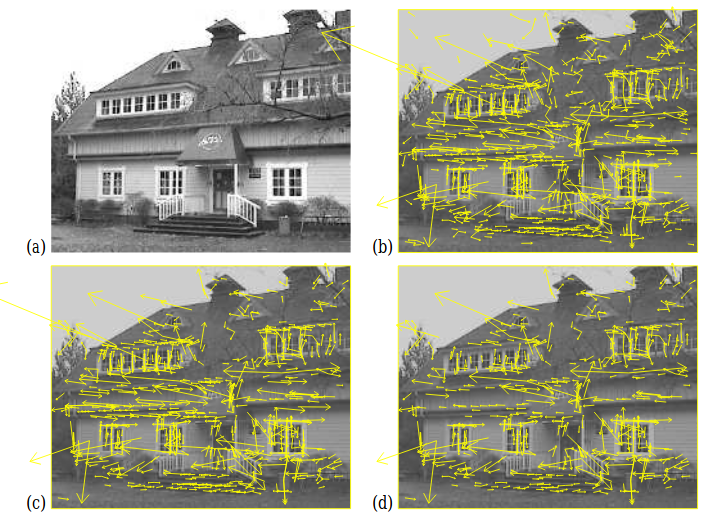
\includegraphics[width=\linewidth]{danhgiakeypoint_quang}
  \caption{Số lượng keypoint còn lại sau khi qua bước 2}
  \label{fig:danhgiakeypoint_quang}
\end{figure}
\subsubsection{Kết luận}
Như vậy, theo hình \ref{fig:danhgiakeypoint_quang} cho ta thấy được: 

- Hình a là ảnh gốc, 233x189 pixel

- Hình b chứa các keypoint sau khi đi qua bước xử lý 1, có 832 keypoint

- Hình c chứa các keypoint sau khi đã bị loại trừ các keypoint có độ tương phản thấp, có 729 keypoint.

- Hình d chứa các keypoint sau khi đã loại bỏ các điểm dư thừa theo biên, còn 536 keypoint.

Như vậy, từ 832 keypoint đã được tìm ở bước 1, thì giờ đây sau khi qua bước 2, ta 
chỉ còn 536 keypoint mà thôi.
 
\subsection{Orientation assignment}
Mục tiêu của phần này là đạt được sự ổn định khi xoay ảnh. Bằng cách gán một hướng duy nhất phù hợp với từng keypoint dựa trên các thuộc tính hình ảnh cục bộ. Các tính toán sử dụng hình ảnh Gaussian mịn $L$ với $scale$ gần nhất. Đối với mỗi hình ảnh mẫu $L(x, y)$, độ lớn gradient $m(x, y)$ và hướng $\theta (x, y)$ được tính toán như sau:
\begin{equation}
\resizebox{1\hsize}{!}{$
m(x,y) = \sqrt{(L(x+1,y) - L(x-1,y))^2 +
 (L(x,y+1)-L(x,y-1))^2}
 $
}%
\end{equation}
\begin{equation}
\theta(x,y) = tan^{-1}(\frac{L(x+1,y) - L(x-1,y)}{L(x+1,y) - L(x-1,y)})
\end{equation}

Một biểu đồ hướng được hình thành từ những hướng dốc của điểm lấy mẫu trong khu vực xung quanh các keypoint. Hướng biểu đồ có 36 ngăn bao phủ $360$ độ. Mỗi mẫu thêm vào biểu đồ được gán trọng số bằng độ lớn gradient của nó và bởi một hình tròn trọng số Gaussian với $\sigma$ gấp $1.5$ lần so với $scale$ của keypoint.
    Các đỉnh tròng biểu đồ định hướng tương ứng với các hướng ưu tiên của cá gradient cục bộ. Đỉnh cao nhất trong biểu đò được phát hiện đầu tiên, và sau đó bất kỳ đỉnh local nào khác trong phạm vi 80$\%$ đỉnh cao nhất được sử dụng để tạo ra một keypoint với hướng đó. Do đó, đối với các vị trí có nhiều đỉnh có cũng độ lớn, sẽ có nhiều keypoint được tạo ra tại một vị trí và tỷ lệ nhưng hướng khác nhau. Chỉ có 15$\%$ số điểm được chỉ định nhiều hướng, nhưng chúng đóng góp đáng kể vào sự chính xác xủa nhận dạng (hình \ref{fig:bieudohuong_tinh})
    
\begin{figure}
  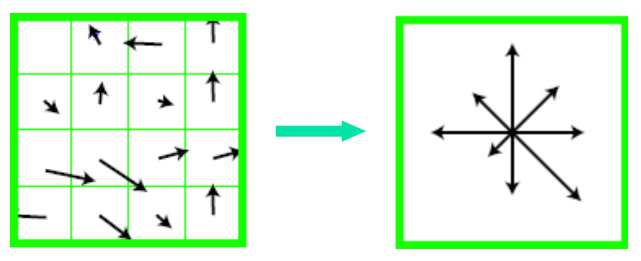
\includegraphics[width=\linewidth]{bieudohuong_tinh}
  \caption{Biểu đồ hướng hình thành từ khu vực xung quanh}
  \label{fig:bieudohuong_tinh}
\end{figure}

\subsection{Keypoint descriptor}
Bước này là để tạo một “dấu vân tay” cho mỗi điểm chính. Điều này giúp xác định một điểm chính. Nếu mắt là một điểm then chốt, sau đó sử dụng “dấu vân tay” này, chúng ta sẽ có thể phân biệt nó với các điểm quan trọng khác, như tai, mũi,...
Để làm điều này, một cửa sổ $16x16$ xung quanh điểm chính được lấy. Cửa sổ $16x16$ này được chia thành $16$ cửa sổ $4x4$. 

Trong mỗi cửa sổ 4x4, độ lớn và hướng của gradient được tính toán.
 Những định hướng này được đưa vào biểu đồ 8 hướng. (hình \ref{fig:tamhuong_phuong})
\begin{figure}
  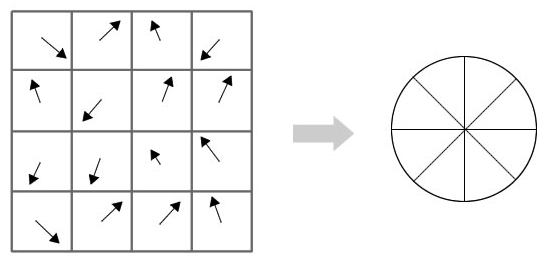
\includegraphics[width=\linewidth]{tamhuong_phuong}
  \caption{Biểu diễn 1 cell $4x4$ thành vector 8 chiều }
  \label{fig:tamhuong_phuong}
\end{figure}

Bất kỳ hướng của gradient nào trong khoảng $0^o-44^o$ thêm vào hướng đầu tiên, tiếp tục cho khoảng $45^o-89^o,90^o-134^o,135^o-179^o,$… Lượng thêm vào mỗi hướng phụ thuộc độ lớn và khoảng cách đến keypoint của gradient.
Điều này được thực hiện bằng cách sử dụng hàm trọng số Gaussian.
Làm điều này cho tất cả $16$ $pixel$, ta sẽ nhận được biểu đồ 8 hướng. Tương tự cho 16 cửa sổ $4x4$. Khi kết thúc, ta sẽ được 1 vector có $4x4x8 = 128$ phần tử. Sau đó chuẩn hóa nó (lấy từng phần tử chia cho độ lớn vector), ta được vector đặc trưng- chính là “dấu vân tay” của điểm chính. (Hình \ref{fig:hinh3_phuong})
\begin{figure}
  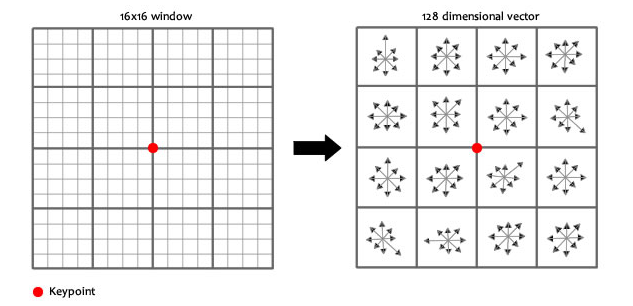
\includegraphics[width=\linewidth]{hinh3_phuong}
  \caption{Biểu diễn 1 cửa sổ $16x16$ thành descriptor 128 chiều}
  \label{fig:hinh3_phuong}
\end{figure}

Một vài biến chứng mà chúng ta cần loại bỏ chúng trước khi hoàn tất “dấu vân tay”
\subsubsection{Sự phụ thuộc vòng quay}vector tính năng sử dụng định hướng gradient. Rõ ràng, nếu bạn xoay hình ảnh, mọi thứ sẽ thay đổi. Tất cả các định hướng gradient cũng thay đổi. Để đạt được sự độc lập xoay, vòng xoay của điểm then chốt được trừ ra khỏi mỗi hướng. Do đó, hướng của mỗi gradient đều liên quan đến định hướng của điểm chính.
\subsubsection{Sự phụ thuộc chiếu sáng}Nếu ngưỡng số liệu mà lớn, chúng ta có thể đạt được sự độc lập chiếu sáng. Vì vậy, bất kỳ số nào (trong số 128) lớn hơn 0,2 sẽ được thay đổi thành 0,2. Sau đó chuẩn hóa vector này lần nữa. Và bây giờ bạn có một vector tính năng độc lập chiếu sáng!
%------------------------------------------------------------------------------
%------------------------------------------------------------------------------
\medskip
\section{PHƯƠNG PHÁP KHỚP NỐI ĐIỂM KEYPOINT}
\label{Sec:PhuongPhapMatching}
Sau khi các keypoint được xác định được các thông số vị trí, tỉ lệ và hướng. Tiếp theo là giai đoạn tuyên quyết để nhận dạng ảnh đó là đối chiếu để tìm ra bức ảnh cần nhận dạng so với ảnh mẫu đưa vào.
\subsection{Khớp keypoint}
Đối sánh các keypoint tốt nhất được tìm thấy bằng cách xác định điểm hàng xóm gần nhất với nó trong cơ sở dữ liệu của keypoint từ hình ảnh huấn luyện. Điểm hàng xóm gần nhất được định nghĩa là các keypoint với khoảng cách Euclide tối thiểu đối với các vector mô tả bất biến.

Khoảng cách $Euclide$:
\begin{equation}
d_{st} = \sqrt{(x_s - y_t)(x_s - y_t)'}
\end{equation}
Nếu khoảng cách bé hơn giá trị THRESHOLD nào đó 
thì chấp nhận. (Hình \ref{fig:khoangcach_nam})
\begin{figure}
  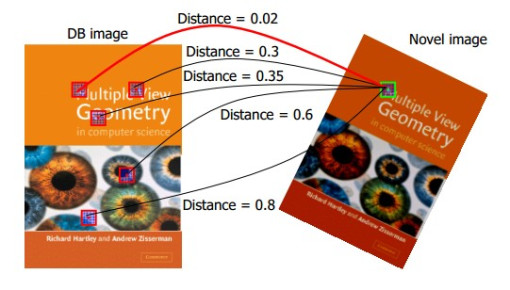
\includegraphics[width=\linewidth]{khoangcach_nam}
  \caption{Ngưỡng chấp nhận của khoảng cách Euclide}
  \label{fig:khoangcach_nam}
\end{figure}

Biện pháp hiệu quả hơn thu được bằng cách so sánh khoảng cách của những điểm hàng xóm gần nhất đó với điểm hàng xóm gần nhất thứ hai. Nếu có nhiều hình ảnh huấn luyện của cùng một đối tượng, ta sẽ định nghĩa điểm hàng xóm thứ hai từ hàng xóm gần nhất được biết đến từ một đối tượng khác so với đối tượng đầu, chẳng hạn như bằng cách chỉ sử dụng các hình ảnh có chứa nhiều đối tượng khác nhau. Biện pháp này hoạt động tốt vì các đối sánh chính xác cần phải có số lượng đáng kể những điểm hàng xóm gần nhất hơn so với đối sánh không chính xác để đạt được đối sánh đáng tin cậy.

Các thao tác trước đó đã được gán một vị trí ảnh, tỉ lệ và hướng đến mỗi điểm Keypoint. Những thông số ám chỉ sự lặp lại vị trí hệ tọa độ $2D$ trong đó mô tả các vùng ảnh cục bộ và do đó bất biến các thông số này. (Hình \ref{fig:soluongkeypoint_nam})

\begin{figure}
  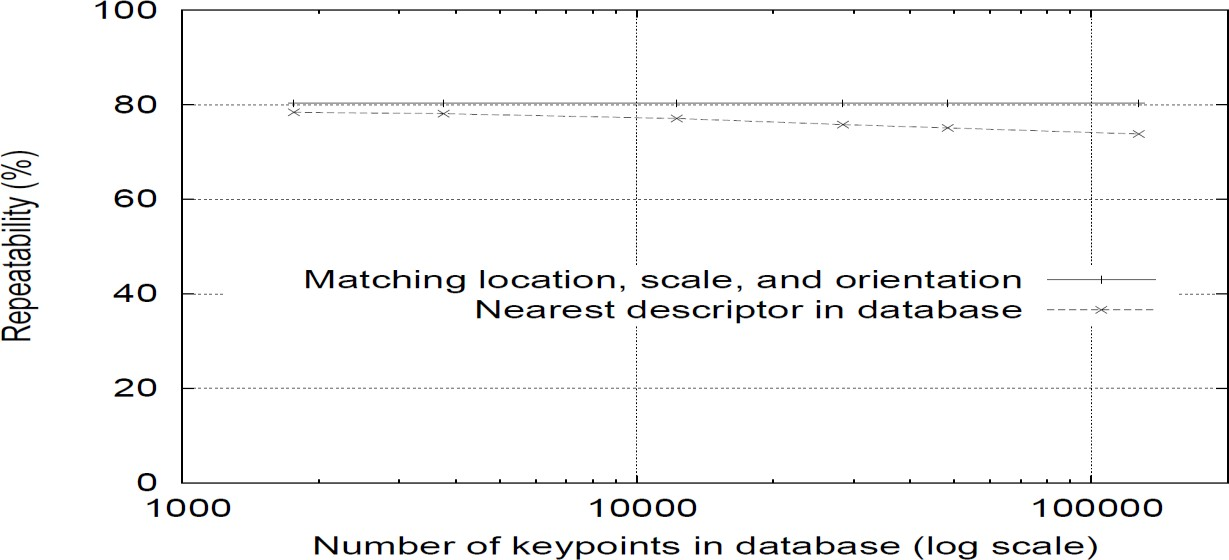
\includegraphics[width=\linewidth]{soluongkeypoint_nam}
  \caption{Số lượng keypoint trong database}
  \label{fig:soluongkeypoint_nam}
\end{figure}
Tỷ lệ phần trăm các keypoint được nhận dạng với số keypoint trong database.

Nét liền là tỷ lệ phần trăm của keypoint được nhận dạng tại vị trí đối sánh đúng và hướng trong hình ảnh chuyển đổi.

Các đường nét đứt hiển thị một phần của thuộc tính ảnh mà những hàng xóm gần nhất trong cơ sở dữ liệu đối sánh đúng như là một hàm của kích thước cơ sở dữ liệu hiển thị trên một tỉ lệ lôgarít (thấy rằng độ tin cậy của đối sánh giảm như là một hàm của số lượng các sai số, nhưng tất cả các dấu hiệu cho thấy nhiều kết quả đúng sẽ tiếp tục được phát hiện ra khi kích thước cơ sở dữ liệu rất lớn).

Vấn đề đặt ra tại sao ta không nhận diện bằng cách tại vị trí đối sánh đúng và hướng mà đôi lúc phải cần nhận diện bằng bộ mô tả descriptor?

Bước tiếp theo là tính toán mô tả cho các khu vực hình ảnh cục bộ mà đặc biệt là chưa bất biến với các biến thể còn lại, chẳng hạn những thay đổi độ sáng hoặc hướng nhìn 3D.
Đây là một vấn đề phức tạp hơn trên.

Khi mà xoay 3D một bức ảnh như vậy thì rõ ràng chúng ta không thể nhận dạng bằng cách trên nữa do vị trí keypoint đã thay đổi tương đôi so với các keypoint cạnh. có một cách khả thi để nhận dạng là dùng bộ mô tả descriptor. (Hình \ref{fig:face3d_nam})

\begin{figure}
  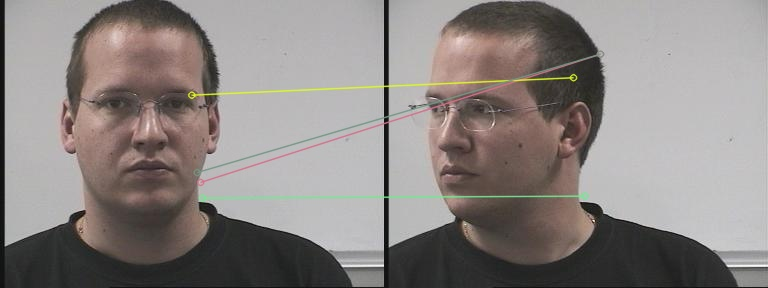
\includegraphics[width=\linewidth]{face3d_nam}
  \caption{Khớp keypoint 3D}
  \label{fig:face3d_nam}
\end{figure}

Khi thay đổi độ sáng trong đó một hằng số được thêm vào mỗi điểm ảnh hình ảnh thì sẽ không ảnh hưởng đến giá trị gradient khi chúng được tính từ sự khác biệt $pixel$. Do đó, các mô tả là bất biến để thay đổi Affine trong chiếu sáng. Tuy nhiên, những thay đổi ánh sáng phi tuyến tính cũng có thể xảy ra do độ bão hòa của máy ảnh hoặc do sự thay đổi ánh sáng có ảnh hưởng đến bề mặt 3D với hướng khác nhau. Các hiệu ứng này có thể gây ra một sự thay đổi tương đối lớn cho một gradient, nhưng ít có khả năng ảnh hưởng đến hướng gradient. Do đó, ta sẽ làm giảm ảnh hưởng của độ dốc lớn bởi các giá trị ngưỡng trong các vector đặc trong cho mỗi đơn vị, ngưỡng này không được lớn hơn $0.2$ và sau đó đưa về giá trị bình thường cho mỗi đơn vị chiều dài. Điều này có nghĩa là sự phù hợp với độ lớn cho gradient không còn là quan trọng và sự phân bố các hướng có trọng tâm hơn. Giá trị của 0.2 được xác định bằng thực nghiệm bằng cách sử dụng các hình ảnh có chứa sự chiếu sáng khác nhau đối với các đối tượng 3D.


%------------------------------------------------------------------------------
% Section 5: Postprocessing
%------------------------------------------------------------------------------
\medskip
\section{Các đặc tính của thuật toán và hệ thống}
\label{Sec:Cacdactinh}
Như các sản phẩm trên thị trường, thuật toán cũng vậy, nó cần có những thông số cụ thể, khách quan qua quá trình chạy thử và kiểm chứng để người sử dụng có thể lựa chọn tối ưu và phát huy cao nhất điểm mạnh của nó. Đối với một thuật toán nhận dạng, những yếu tố cần được quan tâm nhất chính là thời gian xử lý, tỉ lệ chính xác đối với nhiễu, méo, tỷ lệ… và các yếu tố khác.

Sau đây nhóm em xin được trình bày thuật toán được thực hiện trên matlab, với sự tham khảo của \textbf{behindsciences.com} \cite{CodeMatlab}.

\begin{figure}
  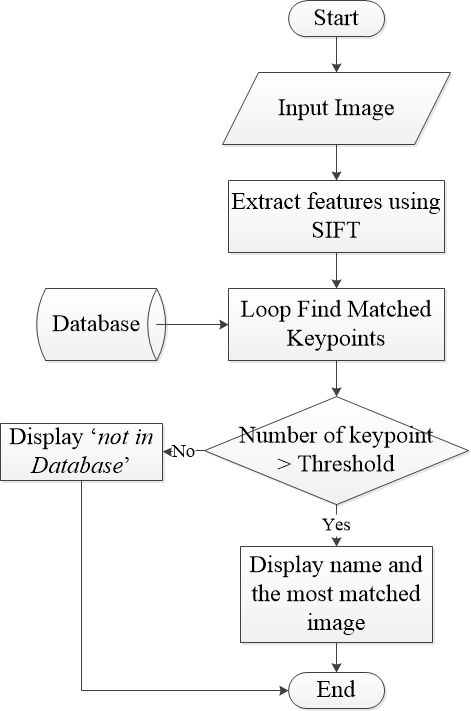
\includegraphics[width=\linewidth]{thuatoan}
  \caption{Thuật toán mô hình chung để nhận dạng mặt}
  \label{fig:thuatoan}
\end{figure}

Dựa vào thuật toán (hình \ref{fig:thuatoan}), tư tưởng cơ bản như sau:

Đầu tiên khởi động chương trình, đặt ảnh cần nhận dạng (gọi là input). Sau đó thuật toán SIFT sẽ trích xuất keypoint từ ảnh input. Kế tiếp đó so sánh keypoint đã có sẵn trong database. Nếu số lượng keypoint trùng khớp lớn hơn một ngưỡng cho phép thì ta nhận dạng thành công và xuất "tên" lên màn hình. Ngược lại, ta xuất "not in database", nghĩa là không có trong database lên màn hình.

Sau đây, nhóm em sẽ đi sâu hơn về quy trình nhận dạng:

\subsection{Thời gian Training}
Thời gian training được tính trên Database AAA$\_$DataLEM với hình số 1 của mỗi người có trong database.

    Đoạn code thực hiện:
    
\begin{lstlisting}
tic;
trainData();
toc;
\end{lstlisting} 

\begin{figure}
  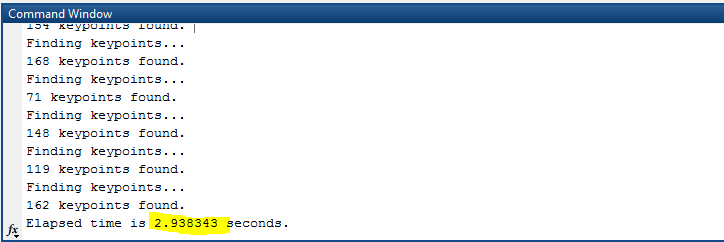
\includegraphics[width=\linewidth]{ketqua1_tinh}
  \caption{Workspace tính thời gian training trung bình}
  \label{fig:ketqua1_tinh}
\end{figure}      
    Kết  quả:
   Sau khi thực hiện đoạn code, ta lấy kết quả thu được chia cho số ảnh training.
   Thời gian training trung bình 1 ảnh: 0.1959s (Hình \ref{fig:ketqua1_tinh})
\subsection{Thời gian nhận dạng}
Các tính toán sau sẽ thực hiện trên Database AR LEM Face với hình số 1 (trong database) của mỗi người và hình số 14 (trong database) (hình chụp người đó sau 2 tuần). Hình số 1 sẽ là hình training và hình số 14 sẽ được dùng để nhận dạng. Cơ sở dữ liệu chứa dữ liệu của 100 người gồm 50 nam và 50 nữ. Ta sẽ tăng dần số số người được training và số người được nhận dạng, sau đó biểu diễn trung bình thời gian nhận dạng trên trục tọa độ, minh họa trong hình \ref{fig:bieudo1_tinh}.
\begin{figure}
  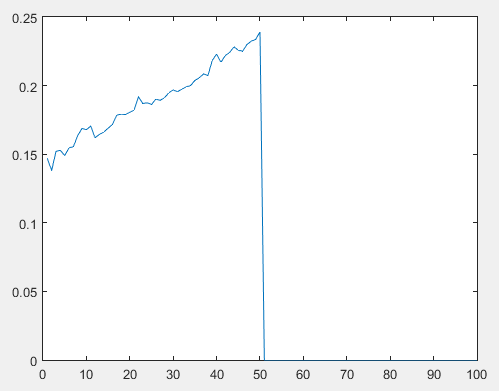
\includegraphics[width=\linewidth]{bieudo1_tinh}
  \caption{Thời gian nhận dạng trung bình một bức ảnh khi Database tăng}
  \label{fig:bieudo1_tinh}
\end{figure} 

Trục tung là thời gian trung bình nhận dạng 1 ảnh, trục dọc là số ảnh có trong file training. Tuy trong cơ sở dữ liệu là 100 người, nhưng ở đây ta chỉ khảo sát đến con số 50 người đầu tiên, lý do vì nếu thực hiện hết 100 người thì số vòng lặp là rất lớn và ý nghĩa của việc này cũng tương đương với 50 người.

\subsection{Lựa chọn mức ngưỡng}
Dùng Database tương tự như phần trước. Tuy nhiên, trong mục này, giá trị của mức ngưỡng sẽ thay đổi theo chiều hướng tăng dần, ta sẽ khảo sát tỷ lệ chính xác của việc nhận dạng đối với hình 50 người. Kết quả mô phỏng như hình \ref{fig:bieudo2_tinh}.
\begin{figure}
  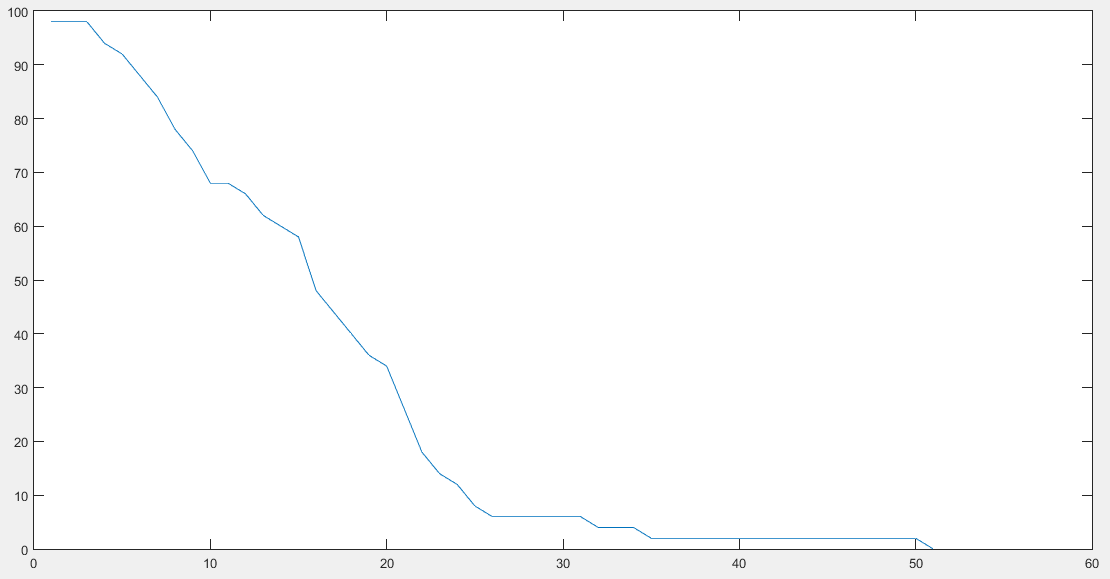
\includegraphics[width=\linewidth]{bieudo2_tinh}
  \caption{Tỷ lệ chính xác của việc nhận dạng khi thay đổi mức ngưỡng}
  \label{fig:bieudo2_tinh}
\end{figure} 

Trục tung của đồ thị trong hình 3 tương ứng với tỷ lệ chính xác của việc nhận dạng, trục hoành sẽ thay đổi theo  $\frac{Threshold}{2} + 1$ (số keypoint giống nhau của hai ảnh phải lớn hơn Threshold thì mới kết luận hai ảnh này là 1).

Tiếp theo, ta khảo sát sự thay đổi của tỷ lệ nhận dạng có ảnh trùng trong database khi mức ngưỡng thay đổi, tức là, dùng ảnh nhận dạng là 50 người nữ trong Database AR LEM Face và ảnh training là 50 người nam trong Database AR LEM Face. Tất yếu, hai tập ảnh hoàn toàn khác nhau nên kết quả cần là giá trị tiến về 0 khi tăng mức ngưỡng. Kết quả minh họa trong hình \ref{fig:bieudo3_tinh}.

Trục tung của đồ thị trong hình \ref{fig:bieudo3_tinh} tương ứng với tỷ lệ có ảnh trùng trong Database, trục hoành sẽ thay đổi theo  $\frac{Threshold}{2} + 1$.

Từ hai kết quả trên, ta sẽ chọn mức ngưỡng phù hợp sao cho tỷ lệ nhận dạng chính xác là cao nhất và tỷ lệ nhận dạng nhầm là thấp nhất. Kết quả là ta có thể chọn mức ngưỡng trong khoảng từ $14\%$ đến $20\%$.

\begin{figure}
  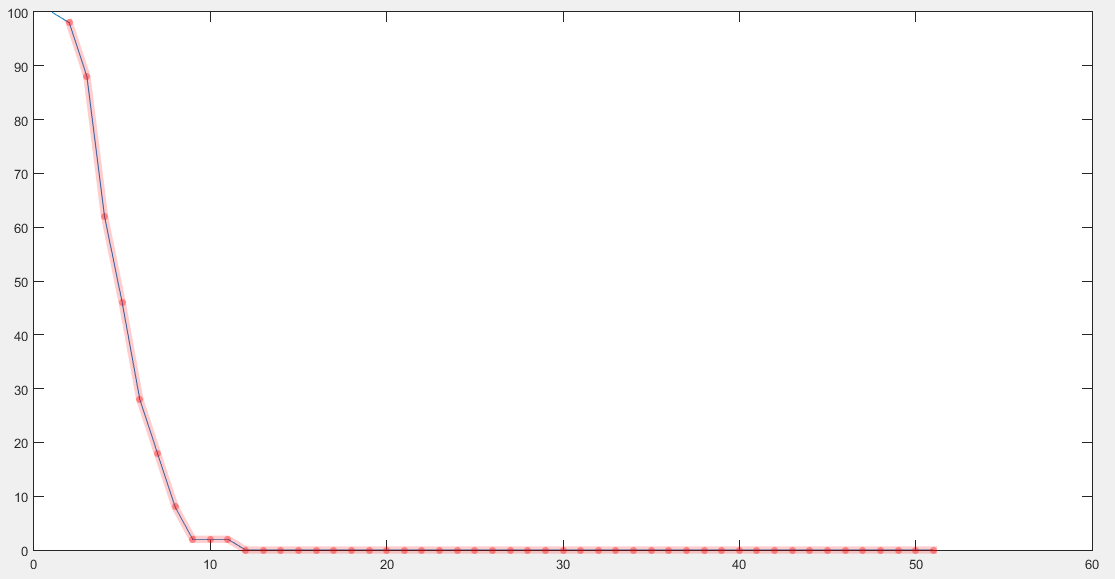
\includegraphics[width=\linewidth]{bieudo3_tinh}
  \caption{Tỷ lệ nhận dạng có ảnh trùng trong Database khi thay đổi mức ngưỡng}
  \label{fig:bieudo3_tinh}
\end{figure} 

\subsection{Nhận dạng trong các điều kiện}
Trong phần này, thực hiện nhận dạng trên Database AAA$\_$DataLEM. Hình được dùng để nhận dạng là Achermann. Hệ thống chọn mức ngưỡng là $15\%$.
\subsubsection{Che khuất}
Thực chất, che khuất là việc nhận dạng trong tình trạng bị mất các keypoint trong vùng che khuất. Vì thế, sự chính xác trong điều kiện này không những phụ thuộc vào so sánh keypoint mà còn phần đa vào mức ngưỡng được lựa chọn.

    Che khuất một phần nhỏ: hệ thống vẫn nhận dạng đúng. (Hình \ref{fig:bieudo4_tinh})
  \begin{figure}
  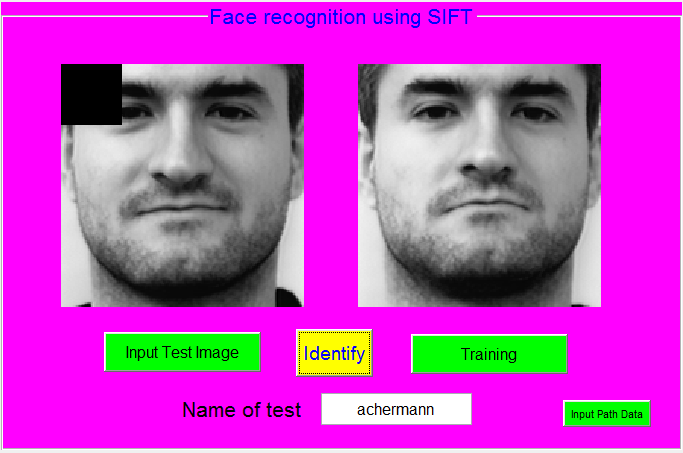
\includegraphics[width=\linewidth]{bieudo4_tinh}
  \caption{Nhận dạng khi bị che khuất (1)}
  \label{fig:bieudo4_tinh}
\end{figure}   

Che khuất phần lớn hơn: hệ thống vẫn nhận dạng đúng. (Hình \ref{fig:bieudo5_tinh})
\begin{figure}
  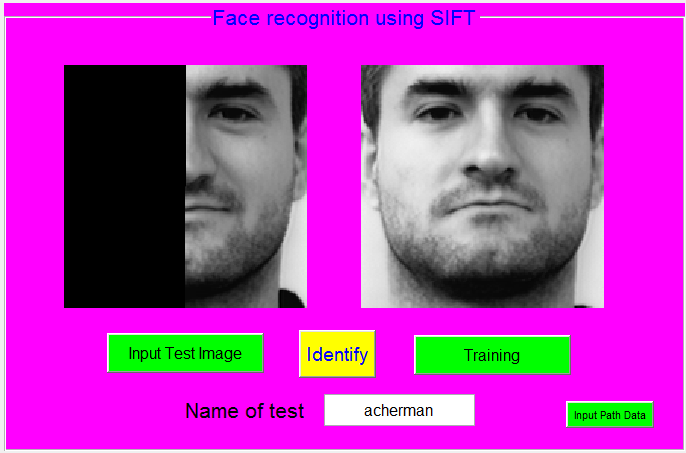
\includegraphics[width=\linewidth]{bieudo5_tinh}
  \caption{Nhận dạng khi bị che khuất (2)}
  \label{fig:bieudo5_tinh}
\end{figure} 
    
    Nhận xét: Thuật toán rất tốt khi nhận dạng ảnh bị che khuất.
    
\subsubsection{Méo dạng}

Thuật toán được khi nhận dạng ảnh bị méo dạng. (Hình \ref{fig:bieudo6_tinh})
\begin{figure}
  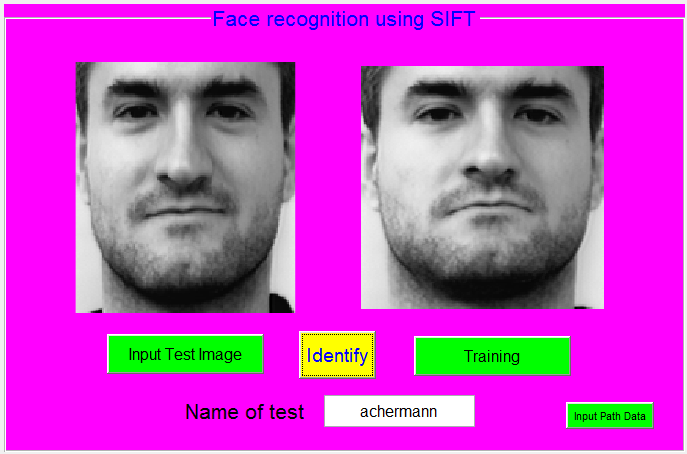
\includegraphics[width=\linewidth]{bieudo6_tinh}
  \caption{Nhận dạng khi bị méo dạng}
  \label{fig:bieudo6_tinh}
\end{figure} 

\subsubsection{Nhiễu}
Hệ thống không thực sự tốt đối với nhiễu, vì vậy cần lọc ảnh có nhiễu trước khi nhận dạng.
(Hình \ref{fig:bieudo7_tinh})
\begin{figure}
  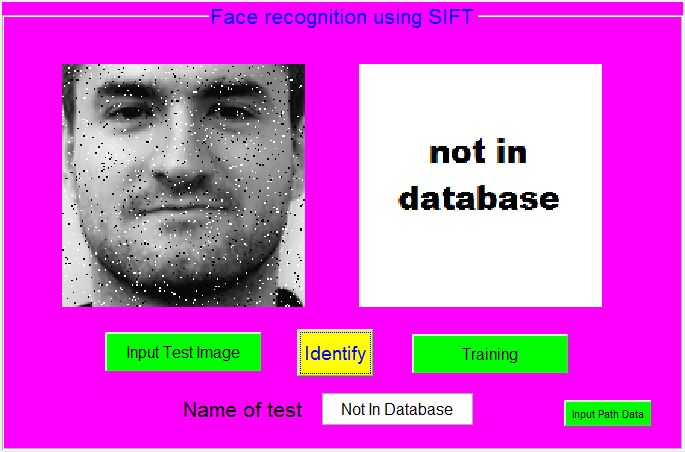
\includegraphics[width=\linewidth]{bieudo7_tinh}
  \caption{Nhận dạng khi bị nhiễu muối tiêu}
  \label{fig:bieudo7_tinh}
\end{figure} 

\subsubsection{Ảnh bị xoay}
Các ảnh sau khi xoay mỗi lần $30^o$ như sau: (Hình \ref{fig:bieudo8_tinh})

Gọi OriginIm là góc ban đầu của bức ảnh. 

Gọi RotateIm là góc xoay của ảnh.

Gọi OriKey  là số keypoint của ảnh gốc.

Gọi RotKey là số keypoint ảnh xoay.

Gọi MatchKey là số keypoint matched.

\begin{figure}
  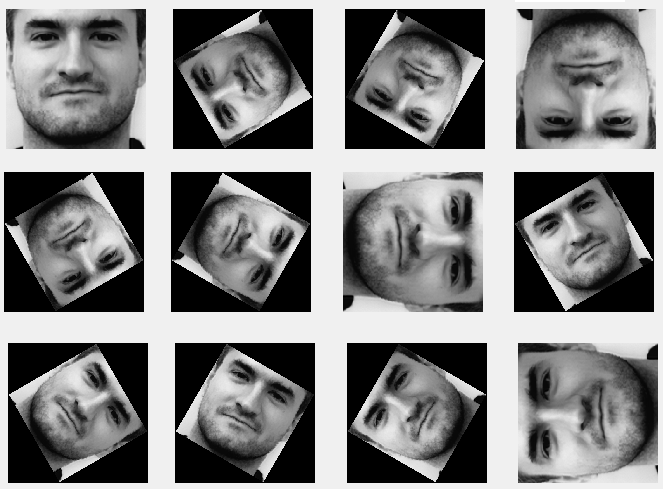
\includegraphics[width=\linewidth]{bieudo8_tinh}
  \caption{Ảnh test sau khi xoay}
  \label{fig:bieudo8_tinh}
\end{figure}

\begin{table}[htb]
\caption{Sự thay đổi số keypoint matched khi xoay ảnh so với ảnh test ban đầu. }
\centering
\label{t:observed_psrs}
\begin{tabular}{ccccc}
\noalign{\smallskip} \hline \hline \noalign{\smallskip
}
OriginIm & RotateIm & OriKey & RotKey & MatchKey \\
\hline
0        & 0$^o$            & 131 	&131		&131 	\\
0        & 30$^o$           & 131 	&123		&62		\\
0        & 60$^o$           & 131 	&130		&63		\\
0        & 90$^o$           & 131 	&127		&120	\\
0        & 120$^o$          & 131 	&121		&61		\\
0        & 150$^o$          & 131 	&131		&67		\\
0		 & 180$^o$			& 131 	&130		&125	\\
0		 & 210$^o$			& 131 	&123		&61		\\
0        & 240$^o$          & 131 	&124		&65		\\
0        & 270$^o$          & 131 	&131		&66		\\
0        & 300$^o$          & 131 	&130		&63		\\
0        & 330$^o$          & 131 	&130		&124	\\


\noalign{\smallskip} \hline \noalign{\smallskip}
\end{tabular}
\end{table}

Nhận xét: Dựa vào bảng \ref{t:observed_psrs} ,so với ảnh ban đầu số keypoint còn tương đương vẫn xấp xỉ 50$\%$. 
%------------------------------------------------------------------------------
% Section 6: Result
%------------------------------------------------------------------------------
\medskip
\section{KẾT LUẬN}
\label{Sec:KetLuan}
\subsection{Kết luận}
Trong mục này, nhóm em đã tìm hiểu được cơ bản thuật toán SIFT cách trích keypoint từ ảnh và mô tả chúng qua vị trí, hướng và độ lớn. Vận dụng thuật toán SIFT thông qua phần mềm MATLAB vào nhận dạng khuôn mặt, đáp ứng được yêu cầu của giáo viên hướng dẫn. Kiểm tra được các đặc tính của thuật toán và hệ thống sử dụng thuật toán để nhận dạng khuôn mặt.

\subsubsection{ƯU ĐIỂM}
Dựa vào những thử nghiệm ở các bước trên, ta có thể nhận xét rằng:

Keypoint phụ thuộc rất ít vào cường độ sáng, che khuất (một phần ảnh bị che), góc xoay (ảnh bị xoay trong mặt phẳng 2D), thay đổi của tư thế (pose thay đổi trong không gian 3D).
\\

\subsubsection{NHƯỢC ĐIỂM}
Theo thử nghiệm ở bước trên, nếu có nhiễu muối tiêu thì việc nhận dạng trở nên khó khăn hơn. Ngoài ra, việc lưu trữ keypoint trong database là rất lớn. Ví dụ, nếu 1 ảnh có 200 keypoints, 10 ảnh là 2000, vậy ta cần train 100 ảnh thì con số rất lớn. Điều đó cũng dẫn đến công đoạn khớp keypoints để nhận dạng, gây ra mất nhiều thời gian hơn!\\


    \subsubsection{Khó khăn gặp phải}Tuy đã tìm hiểu được cơ bản thuật toán SIFT, nhưng để hiểu tường tận nó thì cần có những kiến thức nền vô cùng vững chắc, những kiến thức có trong phần References của bài báo \textbf{“Distinctive Image Features from Scale-Invariant Keypoints”} của tác giả David G. Lowe. Điều này gây rất nhiều khó khăn cho nhóm trong quá trình tìm hiểu các khái niệm và thuật toán liên quan.
\subsection{Hướng phát triển đề tài}
Nhận dạng khuôn mặt realtime: Thời gian nhận dạng trung bình 1 ảnh từ $0.15$ đến $0.2s$, tuy nhiên ta có thể dùng thuật toán song song ($parallel$) chia nhỏ chương trình và thực hiện trên nhiều lõi CPU cùng lúc để tăng tốc độ nhận dạng; cũng có thể kích thước ảnh đến mức phù hợp vừa có thể nhận dạng vừa tăng số keypoint.

    Nhận dạng vật thể: Chúng ta có thể trích đặc trưng của một vật thể thay vì khuôn mặt và nhận dạng chúng trong một $background$ gồm nhiều vật thể khác.

%------------------------------------------------------------------------------
% References
%------------------------------------------------------------------------------
\medskip
\begin{thebibliography}{9}

\bibitem{baibao1}
{Lowe, D. 2004 \textit{"Distinctive image features from scale-invariant keypoints"}, International Journal of Computer Vision, Vol. 60, No. 2, 91–110.}\\

\bibitem{baibao2}
{Brown, M. and Lowe, D.G. 2002.  \textit{"Invariant features from interest point groups"}.  In British Machine Vision Conference, Cardiff, Wales, pp. 656-665.}


\medskip
\bibitem{CodeMatlab}
\url{https://www.mathworks.com/matlabcentral/fileexchange/57033-face-recognition-algorithm-using-sift-features}



\end{thebibliography}


%------------------------------------------------------------------------------
% End of document
%------------------------------------------------------------------------------
\end{document}

